\documentclass[12pt,titlepage]{article}
\usepackage{graphicx} % Required for inserting images
\usepackage{amsmath}
\usepackage{float}
\usepackage{array}
\usepackage{longtable}
\usepackage{booktabs}
\usepackage{tabularray}
\usepackage{biblatex}
\addbibresource{bibliography.bib}
\usepackage{hyperref}
\hypersetup{
    colorlinks,
    citecolor=blue,
    filecolor=black,
    linkcolor=black,
    urlcolor=blue,
    linktoc=all
}
\usepackage[font=small,labelfont=bf]{caption}
\usepackage[a4paper,margin=2cm]{geometry}
\renewcommand{\contentsname}{Contenuti}
\renewcommand{\figurename}{Fig.}
\renewcommand{\arraystretch}{1.25}

\title{Zeldagen}
\author{Daniele De Martino}
\date{9 January, 2025}

\begin{document}

\begin{titlepage}
  \begin{center}
    \centerline{
\includegraphics[height=42mm]{assets/logo-unisa.png}}

    \vspace{0.5cm}
    {\sc {\large Universit\`a degli studi di Salerno} \\ Corso di laurea in Informatica}\\[1em]

    \vspace{1cm}
    {\sc \large Progetto di Fondamenti di Intelligenza Artificiale}

    \vspace{0.2cm}
    \centerline{\hbox to 13cm{\hrulefill}}
    \vspace{0.3cm}
    {\sc \Large {\textbf{Zeldagen}}}
    \centerline{\hbox to 13cm{\hrulefill}}

    \vspace{1.2cm}
    {\sc {\Large Daniele De Martino}\\
    0512116151 \\ [1 cm]
    \large Prof. Fabio Palomba}

    \vspace{3cm}

    \begin{figure}[h]
    \centering
    \begin{minipage}{.5\textwidth}
    \centering
    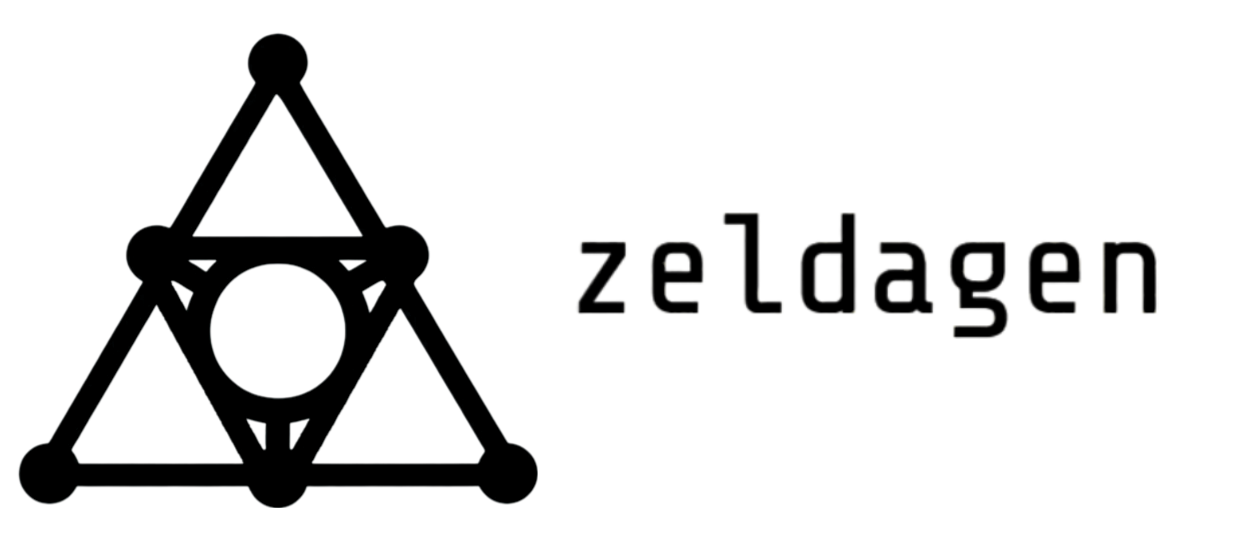
\includegraphics[width=.7\linewidth]{assets/zeldagen-logo-transparent-long.png}
    \end{minipage}%
    \end{figure}

    \vspace{0.3cm}

    \hbox to \textwidth{\hrulefill}
    \vspace{0.2cm}
    {\sc  gennaio, 2025 - anno accademico 2024/2025}

  \end{center}
\end{titlepage}

\newpage
\tableofcontents
\newpage

\section{Introduzione}

\subsection {Premesse}
Il progetto premette la conoscenza di alcune nozioni videoludiche, le quali saranno ora spiegate per permetterne la comprensione. Qualora fossero concetti noti, è possibile saltare questo paragrafo.\\


\noindent Un \textbf{dungeon} (lett. \textit{"prigione"}, \textit{"segreta"}) è un percorso labirintico composto da più ambienti, stanze o livelli, in cui ciascuno di questi presenta pericoli per il giocatore (l'eroe) che lo affronta, come nemici, trappole o enigmi.

Generalmente, i dungeon presentano una o più entrate, una o più uscite, con uno o più \textit{"boss"} (avversari particolarmente difficili da sconfiggere) a guardia delle uscite, e ovviamente numerose porte chiuse, chiavi e tesori da trovare.\\


\noindent Nel contesto della saga \textit{The Legend of Zelda}, generalmente i dungeon sono composti da una sola entrata e una sola uscita, nella quale è posto il boss.

Difficilmente presentano trappole, bensì ogni stanza può presentare enigmi e nemici da sconfiggere (spesso impedendo il prosieguo finché non sconfitti).

Una delle meccaniche più caratteristiche dei dungeon di Zelda è che le stanze sono tra loro connesse tramite porte, che possono a volte essere chiuse a chiave: è quindi necessario trovare le chiavi nei tesori sparsi in giro per il dungeon. Ciascuna chiave può sbloccare qualsiasi porta chiusa si desideri, eccetto la chiave finale, necessaria per sbloccare la stanza d'uscita con il boss.\\

\noindent Questo implica che la navigazione viene solo ``proposta" al giocatore, ed è lui quindi a scegliere come navigare il dungeon, talvolta tornando indietro (effettuando il cosiddetto \textit{backtracking}), utilizzando secondo i propri criteri le chiavi - l'importante è che sia sempre possibile completare il dungeon, a prescindere da come si è scelto di utilizzarle.

\subsection {Panoramica ed obiettivi}
\textit{Zeldagen} è un progetto di generazione procedurale di topologie di dungeon Zelda-like, mediante l'utilizzo di algoritmi genetici (\textit{``gen"} da \textbf{gen}erativo e da \textbf{gen}etico).

\noindent L'idea nasce dal fatto che, tradizionalmente, per ottenere esperienze di gameplay di qualità come quelle della saga videoludica The Legend of Zelda (che ha appassionato milioni di persone negli anni), i requisiti sulle sfide che vengono poste al giocatore sono stringenti: è particolarmente complicato ottenere un dungeon che risulti appagante e bilanciato, senza la progettazione umana.\\

\noindent Difatti, in condizioni normali, tutti i videogiochi che utilizzano un sistema di generazione procedurale, tendono al \textbf{compromesso varietà vs. qualità}: per ottenere esperienze sempre differenti e mai noiose, si è spesso costretti a tralasciare un po' la qualità di tali esperienze.\\

\noindent L'obiettivo del progetto è quindi di ottenere delle topologie di dungeon generate proceduralmente che risultino appaganti per un giocatore umano, allo scopo di poterlo integrare nello sviluppo di videogiochi ed ottenere esperienze sempre nuove e differenti, ma senza tralasciare la qualità.

Ci sono ovviamente molti modi per ottenere questo risultato, ma la proposta di Zeldagen è l'utilizzo di un agente intelligente. La scelta è ricaduta su un algoritmo di IA poiché la conoscenza (personale e collettiva) dell'argomento non è così avanzata da avere euristiche che permettano una efficace ed efficiente generazione senza tanta sperimentazione --- in questo caso quindi è d'aiuto lo sperimentare ed esplorare lo spazio degli stati.

Si è scelto un algoritmo genetico poiché nel problema in esame è molto semplice ottenere un dungeon ``valido", ma è complicato ottenere un dungeon di qualità, ed il modo migliore per farlo è tramite ottimizzazione e raffinamenti successivi.

\section{Descrizione dell'agente}

Lo scopo dell'agente intelligente sarà quindi generare una topologia di dungeon che rispecchi determinate caratteristiche in seguito descritte.

\subsection {Specifica PEAS}

- \textbf{Performance}: la misura di prestazione è la generazione di dungeon risolvibili e quanto più vicini alle \textbf{metriche di validità e di successo} (descritte in seguito);\\
- \textbf{Environment}: lo spazio dei possibili dungeon, in particolare è:\\
\indent --- \textbf{completamente osservabile}: si ha accesso a tutte le caratteristiche che si desidera conoscere dei grafi, a patto di calcolarle (con relativi costi computazionali);\\
\indent- \textbf{deterministico}: è l'agente a determinare come muoversi nell'ambiente;\\
\indent- \textbf{episodico}: l'agente effettua azioni ``atomiche";\\
\indent- \textbf{discreto}: anche se molto ampio, quindi complesso da esplorare tutto;\\
\indent- \textbf{statico};\\
\indent- \textbf{a singolo agente};\\
- \textbf{Actuators}: le possibili modifiche atomiche che l'agente può effettuare su un singolo grafo, in particolare modificando pesi dei nodi, pesi degli archi, o creando, rimuovendo e spostando archi. Non può aggiungere nodi, nel nostro specifico caso;\\
- \textbf{Sensors}: le possibili informazioni che l'agente può determinare sul grafo, tra cui i nodi, gli archi, i pesi di ciascuno di essi, ed eventuali calcoli che può fare in base a questi ultimi (tra cui calcolare la \textbf{fitness}, determinarne la risolvibilità, la difficoltà e così via).

\section{Progettazione}

La parte pregnante del problema è determinare i soggetti su cui stiamo lavorando e determinare delle metriche capaci di misurarne la qualità.

\subsection {Definizione degli individui}

Il soggetto su cui Zeldagen lavora è un dungeon, rappresentabile da un \textbf{grafo connesso non orientato}.
I nodi di questo dungeon rappresentano le stanze, mentre gli archi le porte che le connettono.

Per semplificare il problema, si ignoreranno i nemici, i tesori e gli enigmi, i quali possono essere aggiunti in seguito ad una topologia di dungeon già esistente.\\

\noindent Ciascun nodo (stanza) ha un peso che indica il suo tipo --- le stanze possono essere di vari tipi, ma per semplificare se ne sono identificati 4:\\
- stanza iniziale (\textbf{S});\\
- stanza finale del boss (\textbf{F});\\
- stanza normale (\textbf{N}), che presenta nemici e/o enigmi;\\
- stanza con chiave (\textbf{K}), che presenta un tesoro contenente una chiave.\\
Si definirà $V$ l'insieme dei nodi di un dungeon, e $K \subset V$ il sottoinsieme di nodi di tipo K.\\
Un nodo sarà chiamato \textit{``stanza hub"} se possiede esattamente 4 porte.\\

\noindent Anche ciascun arco (porta) ha un peso che indica se la porta è chiusa a chiave oppure no (rappresentabile da un booleano \textbf{``locked"}).\\
Si definirà $E$ l'insieme degli archi di un dungeon, e $L \subset E$ il sottoinsieme di archi chiusi a chiave.\\

\begin{figure}[H]
    \centering
    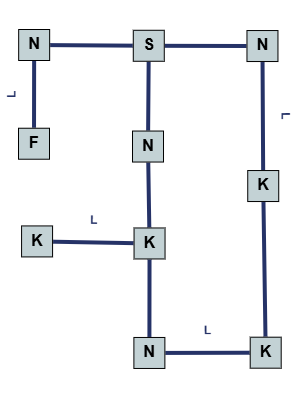
\includegraphics[width=0.33\linewidth]{assets/dungeon-graph-example.png}
    \caption{Rappresentazione grafica di un dungeon}
\end{figure}

\noindent La descrizione precedente si riferisce ovviamente al concetto di dungeon statico, ma non a ciò che avviene quando il dungeon viene ``giocato", il quale presenta un proprio stato, che introduce i concetti di \textbf{chiave} e di \textbf{percorso}.\\

\noindent Il concetto di chiave è rappresentabile con un intero, che indica quante chiavi il giocatore possiede in un dato istante. Attraversare una porta è possibile solo se la porta non è chiusa a chiave, o se è chiusa ma si possiede almeno una chiave per poterla sbloccare --- le porte sbloccate saranno ovviamente aperte per tutto il resto dell'esplorazione.

Le chiavi si ottengono attraversando nodi del tipo chiave (K).\\

\noindent Infine, il concetto di percorso: rappresenta il percorso effettuato finora dal giocatore, il quale partirà sempre dalla stanza iniziale, ed avrà l'obiettivo di raggiungere la stanza finale.

Si noti che si tratta letteralmente di un \textit{percorso} in senso matematico (secondo la teoria dei grafi): una sequenza di vertici $v_0, ..., v_n \in V$, non necessariamente distinti, tutti tra loro connessi da archi $(v_i, v_j) \in E \text{ t.c. } 0 \leq i \neq j \leq n$.

È quindi matematicamente corretto parlare di \textbf{percorso}, ed è da non confondere, ovviamente, con il concetto di \textbf{cammino}.\\

\noindent Si chiamerà \textbf{soluzione} un percorso che risolve il dungeon, rappresentato da una sequenza ordinata di nodi, dove il primo sarà sempre la stanza iniziale e l'ultimo la stanza finale:\\
$\{v0, ..., v_n\} \text{ t.c. } \text{sia un percorso} \, \land \, n \geq 1 \, \land \, type(v_0) = S \, \land \, type(v_n) = F$.\\
Nel contesto del documento, la soluzione migliore (col minor numero di stanze), sarà chiamata $S$.\\

\noindent Seguendo quindi le definizioni appena date, il problema diventa equiparabile alla generazione di labirinti, con il vincolo aggiunto delle chiavi sia durante la generazione che durante il gioco.

\subsection {Metriche di validità e di successo}

Ciò che segue è frutto di una ricerca approfondita su ciò che concerne la giocabilità, la difficoltà ed il buon game design di un dungeon in un gioco in stile Zelda.\cite{metazelda}\cite{hacker}\\

\noindent Le seguenti metriche sono dette di \textbf{validità}, cioè determinano un dungeon accettabile ma non buono:\\
\textbf{1v.} presenta una singola stanza iniziale;\\
\textbf{2v.} presenta una singola stanza finale che corrisponde alla stanza del boss;\\
\textbf{3v.} la stanza finale ha una sola porta, ed è sempre chiusa a chiave;\\
\textbf{4v.} non ci sono stanze senza porte;\\
\textbf{5v.} non ci sono stanze con più di 4 porte;\\
\textbf{6v.} il dungeon è risolvibile (non si può restare bloccati, premettendo che il giocatore sia immortale).\\

\noindent Le seguenti metriche sono dette di \textbf{successo}, cioè determinano la buona qualità di un dungeon:\\
\textbf{1s.} il numero di porte deve essere all'incirca il totale delle stanze + $\frac{1}{3}$:\\
$|E| \approx |V| + \frac{1}{3}$;\\
\textbf{2s.} il numero di porte chiuse deve essere all'incirca $\frac{1}{3}$ del totale delle stanze:\\
$|L| \approx \frac{|V|}{3}$
;\\
\textbf{3s.} il numero di stanze necessarie a risolvere il dungeon è circa metà del numero di stanze totali:\\
$|S| \approx \frac{|V|}{2}$
;\\
\textbf{4s.} la soluzione ideale del dungeon richiede un numero di stanze ripetute pari a circa $\frac{1}{4}$ del numero di stanze totali:\\
$|\{v_i \text{ t.c. appare più volte in } S\}| \approx \frac{|V|}{4}$.\\
\textbf{5s.} il numero di stanze con chiave (K) è all'incirca pari al numero di porte chiuse:\\
$|K| \approx |L|$;\\
\textbf{6s.} la shortest path tra la stanza iniziale e quella finale è almeno 2:\\
$|Dijkstra(S, F)| \geq 2$.\\
\textbf{7s.} la stanza iniziale è connessa al più a 3 porte:\\
$degree(v_0) \leq 3$\\
\textbf{8s.} il numero di \textit{``stanze hub"} è al più $\frac{1}{5}$ del numero di stanze totali:\\
$|\{v_i \in S \text{ t.c. } degree(v_i) = 4\}| \leq \frac{|V|}{5}$\\

\noindent Le metriche \textbf{1s}, \textbf{2s} e \textbf{3s} garantiscono una giusta \textbf{difficoltà}, la metrica \textbf{4s} garantisce una bilanciata \textbf{non-linearità}, e le metriche \textbf{5s}, \textbf{6s}, \textbf{7s} e \textbf{8s} garantiscono che il dungeon sia ragionevole, ben costruito e non confusionario.\\

\noindent Oltre alle metriche precedenti, che descrivono quando il risultato prodotto è valido e di qualità, è importante notare che le prestazioni dell'algoritmo sono cruciali, anzi, forse più importanti della qualità stessa del risultato prodotto.

Il principale obiettivo è che il risultato sia prodotto in tempi ragionevoli per poterlo utilizzare nella generazione in tempo reale all'interno di un videogioco.

\section{Soluzione}

Come già discusso, si è optato per l'utilizzo di un \textbf{algoritmo genetico}, con tutte le scelte che comporta. Saranno ora dettagliatamente esaminate una ad una.

\begin{figure}[h]
    \centering
    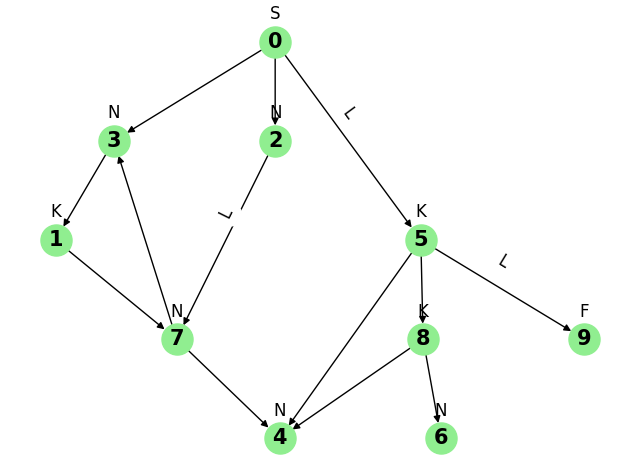
\includegraphics[width=0.65\linewidth]{assets/solution-example.png}
    \caption{Rappresentazione grafica di un individuo soluzione proposto.\\\textbf{Legenda:} S stanza iniziale, F finale, K chiave, N normale, L arco chiuso a chiave.}
\end{figure}

\subsection {Codifica degli individui}

Nonostante avessimo detto che l'individuo per il problema in esame è rappresentato da un grafo \textbf{non orientato}, si è preferito optare nella pratica per un grafo \textbf{orientato}.

Questo ha senso poiché la maggior parte della computazione viene estremamente semplificata se si assume che il grafo abbia un orientamento (ad esempio, è possibile dire che un nodo è una foglia semplicemente vedendo il suo grado uscente), senza perdere alcun vantaggio.

Ovviamente, è necessario convertire il grafo in uno non orientato quando si calcola la risolvibilità e si cerca un percorso soluzione, poiché nel contesto di un videogioco il dungeon è esplorato in modo non orientato. \\

\noindent Per una questione di leggibilità del codice, si è preferito dichiarare gli individui come una classe \textit{Dungeon} con metodi specifici all'algoritmo genetico (es. fitness), permettendo però l'accesso a tutti i metodi diretti sul grafo tramite delegazione (quest'ultimo è gestito dalla libreria \textit{networkx}).

\subsection {Fitness}

La funzione di fitness deriva direttamente dalle \textbf{metriche di validità e successo} identificate nella fase di progettazione.\\

\noindent Le metriche, ora chiamate ``criteri", sono state divise in tre categorie:\\
\textbf{- criteri di validità:} se non rispettati, la fitness risultante è estremamente negativa a prescindere da qualsiasi altro criterio, rendendo l'individuo automaticamente ``scartabile";\\
\textbf{- criteri di penalità:} se non rispettati, la fitness è ridotta in base a un peso;\\
\textbf{- criteri di premialità:} se rispettati, la fitness è incrementata in base a un peso.\\

\noindent Per proseguire con la descrizione dei criteri, è importante far presente che per ciascun individuo valido viene calcolata una soluzione tramite l'algoritmo \textit{shortest path least keys} (approfondito nel successivo paragrafo).

Gli scopi di questa soluzione sono (a) verificare la risolvibilità del dungeon, (b) misurarne la difficoltà, (c) misurarne la non-linearità.

L'algoritmo non è rilevante al puro fine dell'agente intelligente, quindi l'approfondimento del prossimo paragrafo è opzionale. In ogni caso, è necessario sapere che si può assumere che la soluzione prodotta sia la più breve possibile, col minor numero di chiavi, e che consiste in un percorso dalla stanza iniziale a quella finale che rispetti le chiavi e le porte chiuse a chiave.\\

\noindent Saranno ora elencati tutti i criteri calcolati durante la computazione della fitness per ciascun individuo, con relativi premi e penalità.\\

\noindent
\begin{table}[H]
    \centering
    \begin{tblr}{
	vlines = {},
	hlines = {},
        colspec = {Q[c,m]Q[c,m]Q[10cm,l,m]Q[c,m]},
        cell{1}{1} = {c = 4}{halign = c},
        cell{7}{1} = {c = 4}{halign = c}
    }
    \textbf{Criteri di validità} & & & \\
    \textbf{Criterio} & \textbf{Metrica} & \textbf{Descrizione} & \textbf{Fitness} \\
    Validity \#1 & 1v & Il numero di stanze con tipo ``iniziale" deve essere $1$. & $= -100$ \\
    Validity \#2 & 2v & Il numero di stanze con tipo ``finale" deve essere $1$. & $= -100$ \\
    Validity \#3 & 3v & Il numero di archi entranti nella stanza di tipo ``finale" deve essere $1$, e di archi uscenti $0$. & $= -50$ \\
    Validity \#4 & 6v & Deve essere stata trovata una qualunque soluzione mediante l'algoritmo \textit{shortest path least keys}. & $= -100$ \\
    \parbox[c][1cm][t]{\dimexpr\linewidth-2\tabcolsep} {\vspace{0.05cm} La metrica 4v non ha corrispondente nella fitness poiché è garantita per il modo in cui è costruito e modificato il grafo. La metrica 5v è stata resa un \textit{criterio di penalità}.} & & & \\
    \end{tblr}
\end{table}

\noindent
\begin{table}[H]
    \centering
    \begin{tblr}{
	vlines = {},
	hlines = {},
        colspec = {Q[c]Q[c]Q[8cm,l]Q[c]},
        cell{1}{1} = {c = 4}{halign = c},
        cell{1-Z}{1-Z} = {valign = m}
    }
    \textbf{Criteri di penalità} & & & \\
    \textbf{Criterio} & \textbf{Metrica} & \textbf{Descrizione} & \textbf{Fitness} \\
    Penalty \#1 & 2s & Si calcola il numero di porte chiuse a chiave, e si sottrae $2$ per ogni porta chiusa a chiave o meno di differenza rispetto a $\frac{1}{3}$ del numero delle stanze. & $-2|\frac{card(V)}{3} - card(L)|$ \\
    Penalty \#2 & 1s & Si sottrae $2$ per ogni porta in più o meno rispetto al numero delle stanze $+ 33\%$. & $-2|card(E) - \frac{4card(V)}{3}|$ \\
    Penalty \#3 & 6s & Si sottrae $15$ se la lunghezza del cammino più breve tra stanza iniziale e finale (ignorando le porte chiuse) calcolato tramite l'algoritmo di Dijkstra è $< 2$. & $-15$ \\
    Penalty \#4 & 7s & Si sottrae $15$ se la stanza di tipo ``iniziale" ha più di $3$ porte (archi entranti e uscenti). & $-15$\\
    Penalty \#5 & 5v & Si sottrae $15$ per ogni stanza con più di $4$ porte (archi entranti e uscenti). & $-15$ \\
    Penalty \#6 & 8s & Si calcola il numero di \textit{``stanze hub"}, e si sottrae $5$ per ogni \textit{``stanza hub"} in più rispetto a $\frac{1}{5}$ del numero delle stanze. & $-5|\frac{card(V)}{5} - \text{num\_hub}|$\\
    \end{tblr}
\end{table}

\noindent
\begin{table}[H]
    \centering
    \begin{tblr}{
	vlines = {},
	hlines = {},
        colspec = {Q[c]Q[c]Q[7cm,l]Q[c]},
        cell{1}{1} = {c = 4}{halign = c},
        cell{1-Z}{1-Z} = {valign = m}
    }
    \textbf{Criteri di premialità} & & & \\
    \textbf{Criterio} & \textbf{Metrica} & \textbf{Descrizione} & \textbf{Fitness} \\
    Reward \#1 & N/A & \textbf{Quantità di porte:} si aggiunge $1$ per ogni vicino di un nodo (sia entrante che uscente). & $+deg(v_i) \, , \, \forall v_i \in V$ \\
    Reward \#2 & 3s & \textbf{Difficoltà bilanciata:} si aggiunge un quantitativo distribuito normalmente che segue il numero di stanze necessarie alla soluzione \textit{shortest path least keys} ($sp$ nella formula) rispetto alla metà del totale delle stanze. & $+5e^{-card(V)\left(\frac{\text{len(sp)} - \frac{card(V)}{2}}{\frac{card(V)}{2}}\right)^2}$
 \\
    Reward \#3 & 4s & \textbf{Non-linearità bilanciata:} si aggiunge un quantitativo distribuito normalmente che segue il \textit{fattore backtracking} ($bf$ nella formula, ossia il numero di stanze uniche ripetute nella soluzione \textit{shortest path least keys}) rispetto a $\frac{1}{4}$ del totale delle stanze. & $+5e^{-\frac{card(V)}{2}\left(\frac{bf - \frac{card(V)}{4}}{\frac{card(V)}{4}}\right)^2}$ \\
    Reward \#4 & 5s & \textbf{Ragionevolezza delle chiavi:} si aggiunge un quantitativo distribuito normalmente che segue il numero di stanze di tipo ``chiave" ($nkr$ nella formula) rispetto al numero di porte chiuse a chiave ($card(L)$). & $+5e^{-card(V)\left(\frac{nkr - card(L)}{card(L)}\right)^2}$ \\
    \end{tblr}
\end{table}

\noindent L'utilizzo delle distribuzioni normali nei criteri di premialità permette di assegnare un certo premio (definito principalmente dal peso per cui si moltiplica la distribuzione) in caso il criterio sia rispettato, sottraendo in modo \textbf{esponenziale} invece per chi non soddisfa tale criterio, andando quindi a penalizzare poco chi vi si avvicina e molto chi vi si allontana.\\

\noindent Dati questi criteri, la fitness calcolata può essere utilizzata per la fase di selezione. Prima di procedere con le ulteriori scelte applicate per la realizzazione dell'algoritmo genetico, però, ci si soffermerà brevemente sull'algoritmo \textit{shortest path least keys} prodotto.

\subsubsection {Algoritmo shortest path least keys}

\textit{Shortest path least keys} (nome ideato ad hoc per il problema in esame) è un algoritmo \textbf{ricorsivo} di \textbf{ricerca non informata}, simile alla \textbf{depth-first search}, che utilizza il \textbf{backtracking}, creato allo scopo di trovare il percorso soluzione ad un dungeon che sia più breve possibile, in termini di nodi del percorso, e che utilizzi il minor numero di chiavi possibile.\\

\noindent L'algoritmo prende in prestito diverse idee dalla DFS, come appunto la ricorsività ed il backtracking, ma anche dagli algoritmi greedy (favorendo in modo greedy il percorso più breve).

Simulando il comportamento di un giocatore perfetto che sta affrontando il dungeon, opera su grafi non orientati, usando le seguenti strutture dati:\\
\textbf{1.} il numero intero di chiavi possedute in un dato istante;\\
\textbf{2.} un insieme di nodi già esplorati e sui quali non si desidera tornare;\\
\textbf{3.} un insieme di archi (porte) sbloccati in precedenza tramite una chiave;\\
\textbf{4.} un insieme di nodi con chiave attraversati, cioè di cui si è presa la chiave;\\
\textbf{5.} il percorso affrontato fino al dato istante.\\
Inoltre, l'algoritmo necessita di poter accedere all'intero grafo, oltre che di sapere da quale nodo partire (quest'ultimo non è sempre il nodo iniziale, come si vedrà in seguito).\\

\noindent L'algoritmo opera esplorando tutti i nodi connessi a quello corrente (eccetto quelli già esplorati), e per ciascuno di essi effettua un ``tentativo" (definito \textit{``branch"} nel codice).

Con ``tentativo" si intende che, se il nodo è raggiungibile, o se è chiuso a chiave ma si possiede almeno una chiave, si tenta di andare in quella direzione effettuando una chiamata ricorsiva che parte dalla nuova stanza, che ha lo scopo di trovare la shortest path a partire da quella (modificando di conseguenza le strutture dati, ad esempio rimuovendo una chiave se è stata utilizzata).

Il tentativo è locale, nel senso che le modifiche alle strutture dati avvengono solo per quel tentativo. Effettuati tutti i possibili tentativi, si prende quello che restituisce il percorso più breve.\\

\noindent Ovviamente, se una delle stanze attraversate è una stanza di tipo chiave, si aggiunge una chiave a quelle possedute. Avere una nuova chiave, però, significa poter sbloccare percorsi bloccati precedentemente trovati, quindi si introduce il backtracking: quando si trova una chiave si permette all'algoritmo anche di tornare indietro (ma solo in quel caso).

Questo comporta la necessità di tracciare le stanze con chiave esplorate in precedenza, per evitare loop di backtracking infiniti quando due stanze con chiave sono adiacenti.

È necessario tracciare anche le porte già sbloccate, al fine di non restare bloccati nel backtracking quando si affrontano archi chiusi a chiave già sbloccati in precedenza.\\

\noindent L'algoritmo termina un tentativo quando raggiunge un vicolo cieco o raggiunge la stanza finale.

Ciò che l'algoritmo restituisce è un percorso dal nodo iniziale a quello finale, potenzialmente il più breve possibile, ottenuto dai vari tentativi effettuati, prendendo in modo greedy il più breve tra tutti quelli valutati.

In caso non ci sia un percorso valido dal nodo iniziale a quello finale (cioè l'algoritmo a un certo punto non ha più trovato tentativi con cui proseguire), sarà restituito un percorso vuoto, indicante che il dungeon non può essere risolto.\\

\noindent Sebbene il nome, non si garantisce né si è voluto dimostrare in alcun modo che la soluzione prodotta sia la più breve o col minor numero di chiavi possibile, anche se varie sperimentazioni manuali dimostrano che la soluzione, nel caso dei dungeon generati dall'algoritmo, è sempre ottimale.

\subsection {Scelte dei parametri}

\noindent La prima scelta da effettuare è la \textbf{dimensione della popolazione}.

Dopo diverse sperimentazioni, è risultato che una popolazione \textbf{fissa} di \textbf{15 individui} era un ottimo valore, che bilanciava il compromesso tra varietà degli individui e prestazioni dell'algoritmo.\\

\noindent Un'altra scelta importante è il \textbf{il numero di stanze} dei dungeon generati. Questo parametro può variare, e l'algoritmo è stato progettato per funzionare con dungeon con un numero di stanze potenzialmente illimitato, però è stato testato e collaudato solo su topologie di dungeon con \textbf{10 stanze} o \textbf{20 stanze}, poiché è questo il numero di stanze che si vede di solito in un videogioco.

\subsection {Selezione}

Per la fase di selezione è stato provato sia il metodo di \textbf{roulette wheel selection} che il metodo \textbf{k-way tournament} dove $k = \frac{|V|}{4}$, ed i risultati sono stati piuttosto simili; si è pertanto favorito il secondo per aumentare la pressione selettiva (a discapito dell'esplorazione dello spazio degli stati).

\subsection {Cross-over}

È estremamente complesso identificare un metodo di cross-over tra due grafi che mantenga intatte le proprietà migliori di entrambi. Per semplificare le cose, si è preferito evitare cross-over che modificano estensivamente.\\

\noindent La tecnica di cross-over scelta consiste nel generare due figli, che sono cloni rispettivamente di un genitore, ma con due nodi foglia casualmente scambiati (assumendo che un nodo foglia sia un nodo con grado uscente pari a 0).

In realtà, scambiare due foglie, sebbene sia semplice a livello astratto, risulta complesso nel dominio della soluzione (poiché è necessario gestire gli indici che identificano le foglie); nella pratica non si scambiano letteralmente le foglie ma solo i loro dati associati, ossia il tipo di stanza e lo stato di lock di uno dei loro archi entranti.\\

\noindent Questo ci porta ad un meccanismo di cross-over che fa poche e mirate modifiche, in modo efficiente, ma molto aleatorio --- anche se ciò non è necessariamente negativo, e permette di variare molto.

\subsection {Mutazione}

La mutazione è la fase più semplice del problema in esame, poiché ci sono tante possibili modifiche semplici, mirate e veloci che permettono di esplorare alternative differenti nello spazio degli stati.\\

\noindent Proprio per l'alto numero di possibili modifiche, si è preferito non scegliere una sola tecnica di mutazione, ma una a caso tra le seguenti:\\
\textbf{(a) aggiunta di un arco:} restando entro i vincoli della fitness, si aggiunge un arco a due nodi a caso (che non siano quello iniziale o finale);\\
\textbf{(b) rimozione di un arco:} si rimuove un arco a caso tra due nodi che non siano quello iniziale o finale, assicurandosi che il grafo non si disconnetta (cioè che l'arco non sia un \textit{ponte}), ma ignorando la risolvibilità del dungeon (per una questione di efficienza);\\
\textbf{(c) cambiamento del tipo di una stanza:} si seleziona un nodo a caso, che non sia quello iniziale o finale, e si cambia il suo tipo casualmente in ``stanza normale" o ``stanza con chiave" (può anche coincidere e quindi non effettuare alcuna modifica);\\
\textbf{(d) chiusura/apertura di un lucchetto:} si seleziona un arco a caso, eccetto quello connesso alla stanza finale, e se possibile si scambia da chiuso ad aperto o viceversa, in concomitanza con i vincoli imposti dalla fitness.\\

\noindent In ogni caso, la mutazione non può fallire: se non è possibile effettuare l'azione scelta a caso a causa dei vincoli, ne sarà scelta un'altra casualmente finché la mutazione non avviene.

\subsection {Sostituzione e prestazioni}

Dopo alcune sperimentazioni, è risultato chiaro che per aumentare l'efficienza dell'algoritmo fosse imprescindibile l'utilizzo dell'\textbf{elitarismo}: dato che l'algoritmo è estremamente aleatorio, ha molto più senso conservare gli individui migliori ottenuti nel tempo piuttosto che gettare via tutti i progressi ottenuti per esplorare ancora.\\

\noindent Si è scelto quindi di salvare, ad ogni generazione, un certo numero di individui migliori, \textbf{``elite"}, precisamente \textbf{3 individui}. Tutti gli altri individui vengono invece completamente sostituiti dalla generazione successiva.\\

\noindent Inoltre, poiché la fitness viene calcolata diverse volte a causa della sostituzione con elitarismo ed a causa della selezione, è stato implementato un meccanismo di \textbf{caching della fitness}, per evitare di doverne rieffettuare la costosa computazione ogni volta.

\section{Benchmark e considerazioni}

Poiché molte delle scelte relative all'algoritmo sono state effettuate empiricamente, si è dimostrato necessario realizzare numerosi benchmark e misurazioni per valutare quali metodi funzionino meglio.\\

\noindent In questa sezione non si vuole fare una disamina di tutto ciò che è stato valutato e provato, bensì valutare l'algoritmo nel suo stato conclusivo, determinando cosa è andato bene, cosa si sarebbe potuto fare meglio, qual è la qualità dei risultati e le prestazioni.

\subsection {Scelta della tecnica}

La prima considerazione che si vuole effettuare è la tecnica scelta. L'obiettivo del progetto era sfruttare l'intelligenza artificiale nel campo della generazione procedurale, un ambito che non è nuovo nell'utilizzare l'IA ma favorisce algoritmi più veloci rispetto agli algoritmi genetici.\\

\noindent La scelta di un algoritmo genetico non ha portato a una semplificazione del lavoro, anzi: è indubbio che gestire i grafi è estremamente complesso, e a conti fatti sarebbe stato più semplice (a) utilizzare un'altra rappresentazione (motivi approfonditi nel paragrafo 6.1 demo) e (b) approfondire su tecniche di cross-over più avanzate rispetto al semplice scambio di due foglie.\\

\noindent Inoltre, a conti fatti, la difficoltà di progettazione dell'algoritmo genetico è probabilmente la stessa che si avrebbe nel provare a progettare un algoritmo non d'intelligenza artificiale che realizza un dungeon a partire dagli stessi criteri.

\subsection {Risultati}

I risultati ottenuti sono \textbf{ottimi}. Gli individui rappresentano quasi sempre ciò che si desidera ottenere, raggiungendo velocemente una fitness elevata.\\

\begin{figure}
    \centering
    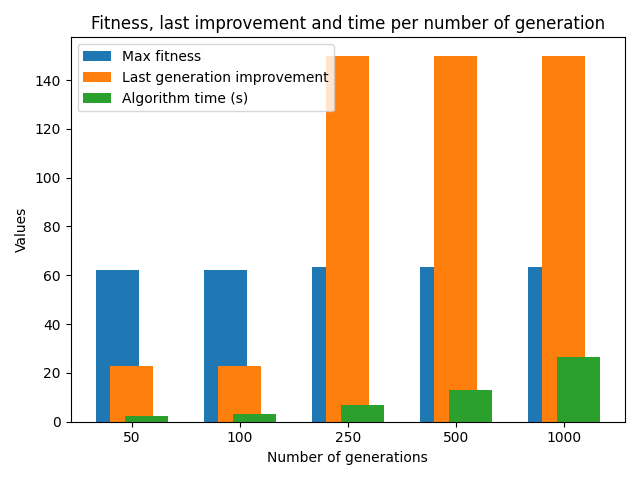
\includegraphics[width=0.75\linewidth]{assets/benchmark.png}
    \caption{Risultati dei benchmark}
\end{figure}

\noindent Come si può osservare in fig. 3 (sotto) dai benchmark prodotti e riesaminati con diversi seed sempre sulla stessa macchina, il risultato è già ottimo nelle prime 50 generazioni (avvicinandosi ad una fitness quasi massima), producendo l'ultimo miglioramento circa alla 23° generazione. Il tempo è molto basso, 1.5 secondi nel caso di 50 generazioni e 3.3 secondi con 100 generazioni.\\

\noindent Però, alla 144° generazione, si ottiene un ulteriore lieve miglioramento (circa 1 punto di fitness in più), arrivando a circa 8 secondi di esecuzione. Oltre la 144° generazione, non si ottengono miglioramenti, delineando la soglia delle 250 generazioni totali come (generalmente) la soglia che ottiene la massima qualità col minimo tempo.\\

\noindent La cosa interessante è che si ottengono risultati circa simili qualunque sia il seed provato, ovvero risultati estremamente buoni sono ottenuti già entro le prime 50 generazioni, e solo raramente si ottengono risultati migliori oltre le 250 generazioni, e solo in casi ancora più rari oltre le 500.\\

\noindent Questo ci porta a pensare che probabilmente l'algoritmo converge molto velocemente, e lo osserviamo indipendentemente dalla pressione selettiva: la ragione potenziale è che il problema è troppo semplice, o troppo restrittivo nonostante sia dettato dal caso, per cui l'algoritmo genetico riesce a risolverlo molto in fretta, ed è possibile che l'utilizzo di un algoritmo genetico sia eccessivo. Si può supporre una corretta modellazione del problema, però applicando tecniche errate per risolverlo.

Allo stesso tempo, non è tutto solo un male: i risultati prodotti sono di buona qualità ed in tempi estremamente brevi, e questo era ciò che si desiderava ottenere.\\

\noindent È interessante notare che la maggior parte del tempo di esecuzione è dovuto al calcolo della fitness, a causa dell'algoritmo \textit{shortest path least keys} e dell'\textit{algoritmo di Dijkstra}.

\section{Note finali}

\subsection {Demo}

L'idea originale per la demo del progetto era di produrre una rappresentazione grafica dei dungeon, simile ad una mappa in un videogioco della serie \textit{The Legend of Zelda}.

Dopo diverse ricerche, però, è risultato che ottenere una rappresentazione di questo tipo a partire da un grafo è molto più complesso del previsto.

Nella ricerca è risultato un concetto matematico interessante: la \textbf{dissezione rettangolare} e la costruzione di \textbf{rectangular duals} di un grafo, abbastanza simili alla rappresentazione che vogliamo ottenere; diversi risultati scientifici dimostrano che per rappresentare un grafo su un piano (ottenendo un \textit{rectangular dual}) è necessario che si tratti di un \textbf{grafo planare}.

Insomma, la questione è ostica, e a conti fatti non tutti i grafi generati dall'algoritmo sono dimostrabili come planari né è facile applicare un algoritmo che faccia al caso nostro (anche se esiste\cite{bhasker}). Pertanto, l'idea della rappresentazione grafica è stata scartata.\\

\noindent L'idea che si è deciso di applicare per la demo è un sistema di gameplay, mediante gioco di ruolo testuale, di un dungeon generato dall'algoritmo, utilizzando un LLM come narratore.

In questo sistema, l'LLM narra al giocatore testualmente la stanza in cui si trova, narrando eventuali incontri con nemici e tesori, oltre che l'ambiente circostante, integrando nemici e concetti tipici della saga \textit{The Legend of Zelda}.

Il giocatore, invece, ha la possibilità di scegliere le porte da aprire tra le possibili (e quindi la navigazione), con lo scopo di completare il dungeon.\\

\noindent Nonostante l'LLM funga da narratore interattivo, lo stato del gioco è gestito dal programma demo e non dall'LLM, per permettere un gioco coerente ed evitare allucinazioni o dimenticanze.

Nello stato del gioco è compreso il cammino effettuato fino a un dato momento, le chiavi trovate, le porte sbloccate, la salute del giocatore, il possesso della mappa (avere la mappa comporta poter vedere una rappresentazione dell'intero grafo).

Ad ogni azione del giocatore, una parte dello stato del gioco viene comunicata al LLM per permettere  coerenza nelle risposte.\\

\noindent Nella pratica, questo si traduce in una sequenza in cui viene inviato un prompt al LLM, comunicandogli ogni volta le regole del gioco, la stanza in cui il giocatore si trova (con il relativo tipo), le stanze visitabili e la salute del giocatore.

In risposta, l'LLM narra la stanza in cui il giocatore si trova e gli incontri effettuati. Inoltre, comunica quanta salute il giocatore ha perso dopo una battaglia, e/o quante rupie (la valuta della saga \textit{The Legend of Zelda}) ha trovato. In base alla risposta, quindi, viene aggiornato lo stato di gioco dal programma demo.

Una volta letta la descrizione narrativa del LLM, il giocatore può scegliere quale stanza visitare tra le possibili (dettate dal programma) in concomitanza con le proprie chiavi, proseguendo quindi col percorso. La sequenza ricomincia, il prompt viene reinviato e si attende ancora la narrazione.

Il gioco termina quando il giocatore raggiunge la stanza finale e sconfigge il boss, o perde tutta la salute a causa di uno scontro.\\

\noindent Il programma è stato realizzato come \textit{TUI (terminal user interface)}, accessibile cioè tramite un qualsiasi terminale. Utilizza la libreria \textit{Textual} per gestire l'interfaccia e il flusso di controllo.

Per la narrazione, utilizza \textit{Ollama}, in particolare il modello GPT \textbf{LLaMa 3.2} di Meta.

Il vantaggio di Ollama è che può essere eseguito su macchine locali del tutto gratuitamente, a patto di avere risorse sufficienti. Va però installato, prima di poter eseguire la demo.\\

\noindent Il programma demo è solo esemplificativo e non è stato particolarmente raffinato, per una questione di tempi. Pertanto, la qualità del codice lascia a desiderare e potrebbero essere presenti bug.

Anche il prompt utilizzato non è di buona qualità, esente da tecniche di prompt engineering e testing approfondito.

\subsection {Conclusione}

Dal progetto si è tratto un agente intelligente capace di generare proceduralmente topologie di dungeon interessanti per lo sviluppo di videogiochi, generati in tempi estremamente rapidi, e che rispettano regole di game design ben precise.

Grazie alla semplicità degli algoritmi genetici, è molto facile introdurre nuovi vincoli nella funzione di fitness, aderendo ad ulteriori regole.\\

\noindent Il risultato ottenuto è di qualità, anche se sarebbe stato probabilmente possibile utilizzare qualsiasi altro algoritmo di ricerca locale senza troppe differenze.

\subsection {Bibliografia e riferimenti}

I riferimenti bibliografici e non utilizzati nella stesura di questo documento includono due articoli analizzati, e un progetto simile (fonte d'ispirazione) analizzato.

\printbibliography[heading=none]

\end{document}